%$HeadURL: https://practicas-derive.googlecode.com/svn/trunk/funciones_elementales.tex $
%$LastChangedDate: 2008-11-13 12:37:02 +0100 (jue, 13 nov 2008) $
%$LastChangedRevision: 3 $
%$LastChangedBy: asalber $

\chapter{Derivadas}

\section{Fundamentos teóricos}
El concepto de derivada es uno de los más importantes del Cálculo
pues resulta de gran utilidad en el estudio de funciones y tiene
multitud de aplicaciones. En esta práctica introducimos este
concepto y presentamos algunas de sus aplicaciones, tanto en
funciones de una como de varias variables.

\subsection{Tasas de variación media e instantánea. La derivada}
Cuando queremos conocer la variación que experimenta una función
real $f(x)$ en un intervalo $[a,b]$, se calcula la diferencia
$f(b)-f(a)$ que se conoce como \emph{incremento} de $f$, y se nota
$\Delta f[a,b]$, aunque, a veces, simplemente se escribe $\Delta f$.

En muchas otras ocasiones veces resulta importante comparar la
variación que experimenta la función $f$ con relación a la variación
que experimenta su argumento $x$ en un intervalo $[a,b]$. Si tenemos
en cuenta que $b=a+\Delta x$, esto viene dado por la \emph{tasa de
variación media}, que se define como:

\[
\textrm{TVM} f[a,b]=\textrm{TVM} f[a,a+\Delta x]=\frac{\Delta
f}{\Delta x}=\frac{f(b)-f(a)}{b-a}=\frac{f(a+\Delta x )-f(a)}{\Delta
x}.
\]

También resulta muy común llamar a $\Delta x$ con la letra $h$, por
lo que la expresión anterior queda de la forma:

\[
\textrm{TVM} f[a,b]=\textrm{TVM} f[a,a+h]=\frac{\Delta f}{\Delta
x}=\frac{f(a+h)-f(a)}{h}.
\]

Desde el punto de vista geométrico, la tasa de variación media de
$f$ en el intervalo $[a , a+\Delta x]$ es la pendiente de la recta
secante a $f$ en los puntos $(a , f(a))$ y $(a+\Delta x, f(a+\Delta
x))$, tal y como se muestra en la figura~\ref{g:secante}.

\begin{figure}[h!]
\begin{center}
\scalebox{1}{\psset{unit=1.2,xunit=2, ticksize=-3pt 0, algebraic}
\begin{pspicture*}(-1,-0.5)(3.5,4)
\footnotesize
\psaxes[arrows=<->,ticks=none](0,0)(-0.3,-0.3)(2.5,4)
\psplot[linecolor=blue]{0.2}{1.8}{x^3-x^2+x+0.5}
\rput[r](1.4,3.5){$f(x)$}
\psxTick(0.5){a}
\psxTick(1.5){a+\Delta x}
\psline[linewidth=0.5pt,linestyle=dashed,linecolor=gray](0.5,0)(0.5,0.875)
\psline[linewidth=0.5pt,linestyle=dashed,linecolor=gray](1.5,0.875)(0,0.875)
\psline[linewidth=0.5pt,linestyle=dashed,linecolor=gray](1.5,0)(1.5,3.125)(0,3.125)
\psyTick(0.875){f(a)}
\psyTick(3.125){f(a+\Delta x}
\psplot[linecolor=red]{0.2}{1.8}{2.25*x-0.25}
\psline[arrows=|*-|*,linecolor=green](1.5,3.125)(1.5,0.875)
\psline[arrows=|*-|*,linecolor=green](0.5,0.875)(1.5,0.875)
\rput[l](1.6,2){$\Delta y=f(a+\Delta x)-f(a)$}
\rput[t](1,0.8){$\Delta x$}
\end{pspicture*}}
\caption{La tasa de variación media como la pendiente de la recta
secante a una función en dos puntos.} \label{g:secante}
\end{center}
\end{figure}


Y, a veces, incluso más importante que la tasa de variación media,
es estudiar la tasa de variación que experimenta la función, no en
un intervalo, sino en un punto, tomando para ello límites cuando el
incremento en la variable independiente tiende 0. Definimos la tasa
de variación de una función en un punto $a$, o también tasa de
variación instantánea, a partir de la tasa de variación media de la
función en el intervalo $[a,a+\Delta x]$. Dicha tasa, si existe,
recibe el nombre de \emph{derivada} de la función real $f(x)$ en un
punto $a\in \mathbb{R}$, y se nota como $f'(a)$, o bien
$\dfrac{df}{dx}(a)$:

\[
f'(a)=\dfrac{df}{dx}(a)= \lim_{\Delta x\rightarrow 0}\frac{\Delta
f}{\Delta x}=\lim_{\Delta x\rightarrow 0}\frac{f(a+\Delta
x)-f(a)}{\Delta x}=\lim_{h\rightarrow 0}\frac{f(a+h)-f(a)}{h}.
\]

Cuando este límite existe, se dice que la función $f$ es
\emph{derivable} o \emph{diferenciable} en el punto $a$.

Geométricamente, $f'(a)$ es la pendiente de la recta tangente a la
curva de $f(x)$ en el punto $(a,f(a))$, tal y como se aprecia en la
figura~\ref{g:tangente}.

\begin{figure}[h!]
\begin{center}
\scalebox{1}{\psset{unit=1.2,xunit=2, ticksize=-3pt 0, algebraic}
\begin{pspicture*}(-1.5,-0.5)(3,4.5)
\footnotesize
\psaxes[arrows=<->,ticks=none,labels=none](0,0)(-0.3,-0.5)(2,3.5)
\psplot[linecolor=blue]{0.2}{1.5}{x^3-x^2+x+0.5}
\rput[r](1.4,3.5){$f(x)$}
\psxTick(0.5){a}
\psxTick(1.5){x}
\psline[linewidth=0.5pt,linestyle=dashed,linecolor=gray](0.5,0)(0.5,0.875)
\psline[linewidth=0.5pt,linestyle=dashed,linecolor=gray](1.5,0.875)(0,0.875)
\psline[linewidth=0.5pt,linestyle=dashed,linecolor=gray](1.5,0)(1.5,1.625)(0,1.625)
\psyTick(0.875){f(a)}
\psyTick(1.625){f(a)+f'(a)(x-a)}
\psplot[linecolor=red]{0.2}{1.8}{0.75*x+0.5}
\psline[arrows=|*-|*,linecolor=green](1.5,1.625)(1.5,0.875)
\psline[arrows=|*-|*,linecolor=green](0.5,0.875)(1.5,0.875)
\rput[l](1.6,1.25){$f'(a)(x-a)$}
\rput[t](1,0.8){$(x-a)$}
\end{pspicture*}}
\caption{La derivada como la pendiente de la recta tangente a una
función en un punto.} \label{g:tangente}
\end{center}
\end{figure}

\subsubsection*{Recta tangente y normal a una función en un punto}
De la gráfica anterior, fácilmente se deduce que la ecuación de la
recta tangente a una función $f(x)$ en el punto $(a,f(a))$ es:
\[
y=f(a)+f'(a)(x-a).
\]

Y teniendo en cuenta que la pendiente de la recta normal (recta
perpendicular a la recta tangente) es la inversa cambiada de signo,
la ecuación de la recta normal a $f(x)$ en el punto $(a,f(a))$ es:
\[
y=f(a)-\frac{1}{f'(a)}(x-a).
\]

\subsection{Función derivada y derivadas sucesivas}

El límite que nos sirve para calcular la derivada de una función en
un punto, define una nueva función $f'$ cuyo dominio está formado
por los puntos en los que $f$ es diferenciable. La función $f'(x)$,
o también $\dfrac{df}{dx}$, se llama \emph{primera derivada} de $f$.

Puesto que $f'$ es una función, puede derivarse a su vez, y la
primera derivada de $f'$ se conoce como segunda derivada de $f$, y
se nota $f''(x)$ o $\dfrac{d^2f}{dx^2}$. Análogamente, la
\emph{$n$-ésima derivada} de $f$, designada por $f^{(n}$ o
$\dfrac{d^nf}{dx^n}$, es la primera derivada de $f^{(n-1}$, para
$n=2,3,\ldots$, es decir
\[
\frac{d^nf}{dx^n}=\frac{d}{dx}\left(\frac{d^{n-1}f}{dx^{n-1}}\right)\
n=2,3,\ldots
\]


\subsection{Estudio del crecimiento de una función}
Una función $f(x)$ es \emph{creciente} en un intervalo $I$ si
$\forall\, x_1, x_2 \in I$ tales que $x_1<x_2$ se verifica que
$f(x_1)\leq f(x_2)$.

Del mismo modo, se dice que una función $f(x)$ es \emph{decreciente}
en un intervalo $I$ si $\forall\, x_1, x_2 \in I$ tales que
$x_1<x_2$ se verifica que $f(x_1)\geq f(x_2)$. En la
figura~\ref{g:crecimiento_derivada} se muestran estos conceptos.

\begin{figure}[h!]
\centering \subfigure[Función creciente.] {\label{g:funcion_creciente}
\scalebox{1}{\psset{unit=1.5, ticksize=-3pt 0, algebraic}
\begin{pspicture*}(-1,-0.5)(3,2.5)
\footnotesize
\psaxes[arrows=<->,ticks=none,labels=none](0,0)(-0.5,-0.5)(2.5,2.5)
\psplot[linecolor=blue]{0.5}{1.7}{x^1.5}
\psline[linecolor=red,linestyle=dashed](1,0)(1,1)(0,1)
\psline[linecolor=red,linestyle=dashed](1.5,0)(1.5,1.8371)(0,1.8371)
\psxTick(1){x_1}
\rput[t](1.25,-0.1){$<$}
\psxTick(1.5){x_2}
\psyTick(1){f(x_1)}
\rput[r](-0.3,1.415){\rotateleft{$\leq$}}
\psyTick(1.8371){f(x_2)}
\end{pspicture*} }}\qquad
\subfigure[Función decreciente.]{\label{g:funcion_decreciente}
\scalebox{1}{\psset{unit=1.5, ticksize=-3pt 0, algebraic}
\begin{pspicture*}(-1,-0.5)(3,2.5)
\footnotesize
\psaxes[arrows=<->,ticks=none,labels=none](0,0)(-0.5,-0.5)(2.5,2.5)
\psplot[linecolor=blue]{0.5}{1.7}{2.5-x^1.5}
\psline[linecolor=red,linestyle=dashed](0.8,0)(0.8,1.7845)(0,1.7845)
\psline[linecolor=red,linestyle=dashed](1.3,0)(1.3,1.0178)(0,1.0178)
\psxTick(0.8){x_1}
\rput[t](1.05,-0.1){$<$}
\psxTick(1.3){x_2}
\psyTick(1.7845){f(x_1)}
\rput[r](-0.3,1.415){\rotateleft{$\leq$}}
\psyTick(1.0178){f(x_2)}
\end{pspicture*}}}
\caption{Crecimiento de una función.}
\label{g:crecimiento_derivada}
\end{figure}

Si $f$ es una función derivable en el intervalo $I$, el signo de la
derivada puede utilizarse para estudiar el crecimiento de la función
ya que se cumple:
\begin{itemize}
\item $f$ es creciente en $x_0\in I$, si y sólo si, $f'(x_0)\geq 0$.
\item $f$ es decreciente en $x_0\in I$, si y sólo si, $f'(x_0)\leq 0$.
\end{itemize}

Desde el punto de vista geométrico, esto es evidente, ya en los
intervalos donde $f$ es creciente, cualquier recta tangente tiene
pendiente positiva, mientras que en los intervalos donde $f$ es
decreciente, las tangentes tienen pendiente negativa, tal y como se
observa en la figura~\ref{g:crecimiento_derivada}.

\subsection{Determinación de los extremos relativos}
Una función $f(x)$ tiene un \emph{máximo relativo} en $x_0$ si
existe un entorno $A$ de $x_0$ tal que $\forall x \in A$ se verifica
que $f(x)\leq f(x_0)$.

Una función $f(x)$ tiene un \emph{mínimo relativo} en $x_0$ si
existe un entorno $A$ de $x_0$ tal que $\forall x\in A$ se verifica
que $f(x)\geq f(x_0)$.

Diremos que la función $f(x)$ tiene un \emph{extremo relativo} en un
punto si tiene un \emph{máximo o mínimo relativo} en dicho punto.

Cuando $f$ es una función continua, entonces también se puede
definir un extremo relativo como aquel punto donde cambia el
crecimiento de la función. Así, un máximo relativo es un punto donde
la función pasa de ser creciente a ser decreciente, y un mínimo
relativo es un punto donde la función pasa de ser decreciente a ser
creciente, tal y como se muestra en la figura~\ref{g:extremos_derivada}.

\begin{figure}[h!]
\centering \subfigure[Máximo relativo.] {\label{g:maximo}
\scalebox{1}{\psset{unit=1.5, ticksize=-3pt 0, algebraic}
\begin{pspicture*}(-1,-0.5)(3.5,2.5)
\footnotesize
\psaxes[arrows=<->,ticks=none,labels=none](0,0)(-0.5,-0.5)(3.5,2.5)
\psplot[linecolor=blue]{0.5}{3.1}{2-(x-1.8)^2}
\psline[linecolor=red,linestyle=dashed](1.8,0)(1.8,2)(0,2)
\psline[linecolor=red,linestyle=dashed](1,0)(1,1.36)(0,1.36)
\psxTick(1.8){x_0}
\psxTick(1){x}
\psxTick(0.5){x_0-\delta}
\psxTick(3.1){x_0+\delta}
\psyTick(2){f(x_0)}
\psyTick(1.36){f(x)}
\rput[r](-0.3,1.72){\rotateleft{$\leq$}}
\psdot[linecolor=green](1.8,2)
\end{pspicture*}}}\qquad
\subfigure[Mínimo relativo.]{\label{g:minimo}
\scalebox{1}{\psset{unit=1.5, ticksize=-3pt 0, algebraic}
\begin{pspicture*}(-1,-0.5)(3.5,2.5)
\footnotesize
\psaxes[arrows=<->,ticks=none,labels=none](0,0)(-0.5,-0.5)(3.5,2.5)
\psplot[linecolor=blue]{0.5}{3.1}{(x-1.8)^2+0.5}
\psline[linecolor=red,linestyle=dashed](1.8,0)(1.8,0.5)(0,0.5)
\psline[linecolor=red,linestyle=dashed](1,0)(1,1.14)(0,1.14)
\psxTick(1.8){x_0}
\psxTick(1){x}
\psxTick(0.5){x_0-\delta}
\psxTick(3.2){x_0+\delta}
\psyTick(0.5){f(x_0)}
\psyTick(1.14){f(x)}
\rput[r](-0.3,0.8){\rotateleft{$\leq$}}
\psdot[linecolor=green](1.8,0.5)
\end{pspicture*}}}
\caption{Extremos relativos de una función.}
\label{g:extremos_derivada}
\end{figure}

Si $f$ tiene un extremo relativo en un punto $x_0$ y existe la
derivada en dicho punto, entonces se cumple que $f'(x_0)=0$, es
decir, la tangente a la gráfica de $f$ en dicho punto es horizontal
(figura~\ref{g:extremos_derivada}). El recíproco no es cierto en general, de
modo que esta es una condición necesaria pero no suficiente. No
obstante, si $f$ es una función derivable en un intervalo $I$,
podemos utilizar esta propiedad para detectar los puntos entre los
que se encontrarán los extremos relativos del intervalo $I$. Los
puntos donde se anula la primera derivada, se conocen como
\emph{puntos críticos} y serán candidatos a extremos. Una vez
detectados los puntos críticos, para ver si se trata de un extremo
relativo o no, basta con estudiar el crecimiento de la función a la
izquierda y a la derecha del punto tal y como se indicaba en la
sección anterior. Resumiendo, si $f'(x_0)=0$, entonces:
\begin{itemize}
\item Si existe un $\delta>0$ tal que $f'(x)>0\ \forall\, x\in (x_0-\delta,x_0)$ (derivada positiva a la izquierda de $x_0$) y $f'(x)<0\ \forall\, x\in (x_0,x_0+\delta)$ (derivada negativa a la derecha de $x_0$), $x_0$ es un máximo relativo.

\item Si existe un $\delta>0$ tal que $f'(x)<0\ \forall\, x\in (x_0-\delta,x_0)$ (derivada negativa a la izquierda de $x_0$) y $f'(x)>0\ \forall\, x\in (x_0,x_0+\delta)$ (derivada positiva a la derecha de $x_0$), $x_0$ es un mínimo relativo.

\item En cualquier otro, $x_0$ es un \emph{punto de inflexión}.
\end{itemize}

\subsection{Estudio de la concavidad de una función}
Se dice que una función $f(x)$ es \emph{cóncava} en un intervalo $I$
si $\forall\, x_1, x_2 \in I$, el segmento de extremos
$(x_1,f(x_1))$ y $(x_2,f(x_2))$ queda por encima de la gráfica de
$f$.

Análogamente se dirá que es \emph{convexa} si el segmento anterior
queda por debajo de la gráfica de $f$.

Diremos que la función $f(x)$ tiene un \emph{punto de inflexión} en
$x_0$ si en ese punto la función pasa de cóncava a convexa o de
convexa a cóncava. Estos conceptos se ilustran en la
figura~\ref{g:concavidad_derivada}.

\begin{figure}[h!]
\centering \subfigure[Función cóncava.] {\label{g:funcion_concava_arriba}
\scalebox{1}{\psset{unit=1.5, ticksize=-3pt 0, algebraic}
\begin{pspicture*}(-1,-0.5)(3.5,2.5)
\footnotesize
\psaxes[arrows=<->,ticks=none,labels=none](0,0)(-0.5,-0.5)(3.5,2.5)
\psplot[linecolor=blue]{0.5}{3.1}{(x-1.8)^2+0.5}
\psline[linecolor=red,linestyle=dashed](0.9,0)(0.9,1.31)(0,1.31)
\psline[linecolor=red,linestyle=dashed](2.9,0)(2.9,1.71)(0,1.71)
\psline[linecolor=green,arrows=<->](0.9,1.31)(2.9,1.71)
\psxTick(0.9){x_1}
\psxTick(2.9){x_2}
\psyTick(1.31){f(x_1)}
\psyTick(1.71){f(x_2)}
\end{pspicture*}}}\qquad
\subfigure[Función convexa.]{\label{g:funcion_concava_abajo}
\scalebox{1}{\psset{unit=1.5, ticksize=-3pt 0, algebraic}
\begin{pspicture*}(-1,-0.5)(3.5,2.5)
\footnotesize
\psaxes[arrows=<->,ticks=none,labels=none](0,0)(-0.5,-0.5)(3.5,2.5)
\psplot[linecolor=blue]{0.5}{3.1}{2-(x-1.8)^2}
\psline[linecolor=red,linestyle=dashed](0.9,0)(0.9,1.19)(0,1.19)
\psline[linecolor=red,linestyle=dashed](2.9,0)(2.9,0.79)(0,0.79)
\psline[linecolor=green,arrows=<->](0.9,1.19)(2.9,0.79)
\psxTick(0.9){x_1}
\psxTick(2.9){x_2}
\psyTick(1.19){f(x_1)}
\psyTick(0.79){f(x_2)}
\end{pspicture*}}}
\caption{Concavidad de una función.}
\label{g:concavidad_derivada}
\end{figure}


Si $f$ es una función derivable en el intervalo $I$, el signo de la
segunda derivada puede utilizarse para estudiar la concavidad de la
función ya que se cumple:
\begin{itemize}
\item $f$ es cóncava en $x_0\in I$, si y sólo si, $f''(x_0)\geq 0$.
\item $f$ es convexa en $x_0\in I$, si y sólo si, $f''(x_0)\leq 0$.
\end{itemize}


\subsection{Derivadas parciales de una función de $n$ variables}

Recordemos que la derivada de una función de una única variable en
un punto $x=a$ se define como la tasa de variación instantánea de la
función en dicho punto. Si llamamos $h$ al incremento en la
variable, la derivada de la función en $x=a$ se nota como $f'(a)$ ó
$\dfrac{{df}} {{dx}}(a)$, y se calcula como:


\[
f'(a) = \frac{df}{dx}(a) = \mathop {\lim
}\limits_{h \to 0} \frac{{f(a + h) - f(a)}} {h}
\]


Y, en general, para cualquier $x$ en un conjunto en el que la
función de una única variable sea derivable, puede definirse la
función derivada $f'(x)$ ó $\dfrac{df}{dx}$,
mediante el límite:

\[
f'(x) = \frac{df}{dx} = \mathop {\lim }\limits_{h
\to 0} \frac{{f(x + h) - f(x)}} {h}
\]
que, no obstante, se calcula aplicando las adecuadas reglas de
derivación, más bien que acudiendo a la resolución directa del
límite.

De igual forma, si tenemos una función de $n$ variables
$f(\vec{x})=f(x_1,x_2,...,x_n)$, se pueden definir esas mismas tasas
de variación instantáneas con respecto a cada una de las variables
en un punto $\vec{a}=(a_1,a_2,...,a_n)$, para obtener las
\emph{Derivadas Parciales} de la función con respecto a cada una de
las variables en el punto $\vec{x}=\vec{a}$, que se notarán como
$f_{x_i}(\vec{a})$, o bien por $\dfrac{\partial f}{\partial
x_i}(\vec{a})$:



\[
f_{x_i}(\vec{a})=\dfrac{\partial f}{\partial
x_i}(\vec{a})=\lim_{h\rightarrow
0}\frac{f(a_1,\ldots,a_i+h,\ldots,a_n)-f(a_1,\ldots,a_i,\ldots,a_n)}{h},
\]


Y la \emph{Función Derivada Parcial} con respecto a cualquiera de
las variables $x_i$, para todos los $\vec{x}$ de un conjunto, que se
notará como $f_{x_i}$, o $\dfrac{\partial f}{\partial x_i}$:

\[
f_{x_i}=\dfrac{\partial f}{\partial x_i}=\lim_{h\rightarrow
0}\frac{f(x_1,\ldots,x_i+h,\ldots,x_n)-f(x_1,\ldots,x_i,\ldots,x_n)}{h},
\]

Lo cual, a efectos de cálculo, se resume en que la derivada parcial
de una función de varias variables se obtiene como la derivada de
una función de una única variable, que es aquella con respecto a la
que se deriva, y constantes el resto. Como consecuencia, las reglas
de derivación también se aplican en el cálculo de las derivadas
parciales de este tipo de funciones, sin más que considerar
constantes todas las variables con respecto a las que no estamos
derivando.

Si para las funciones de una variable la derivada en un punto $a$
tiene una interpretación gráfica sencilla como la pendiente de la
recta tangente a la gráfica de la función en el punto $(a,f(a))$,
también para funciones de dos variables la derivada parcial con
respecto a $x$ en el punto $\vec{a}=(x_0,y_0)$:

\[
\frac{{\partial f}} {{\partial x}}(x_0 ,y_0 ) = \mathop {\lim
}\limits_{h \to 0} \frac{{f(x_0  + h,y_0 ) - f(x_0 ,y_0 )}} {h}
\]
representa la pendiente de la recta tangente a la curva que se
obtiene al cortar la gráfica de la función en el punto
$(x_0,y_0,z_0=f(x_0,y_0))$ mediante el plano en el que $y$ permanece
constante e igual a $y_0$, y tan sólo varía el valor de $x$. E
igualmente, la derivada parcial con respecto a $y$ será la pendiente
de la recta tangente a la curva que se obtiene al cortar la gráfica
de la función en $(x_0,y_0,z_0=f(x_0,y_0))$ mediante el plano
$x=x_0$.

\begin{figure}[h!]
\begin{center}
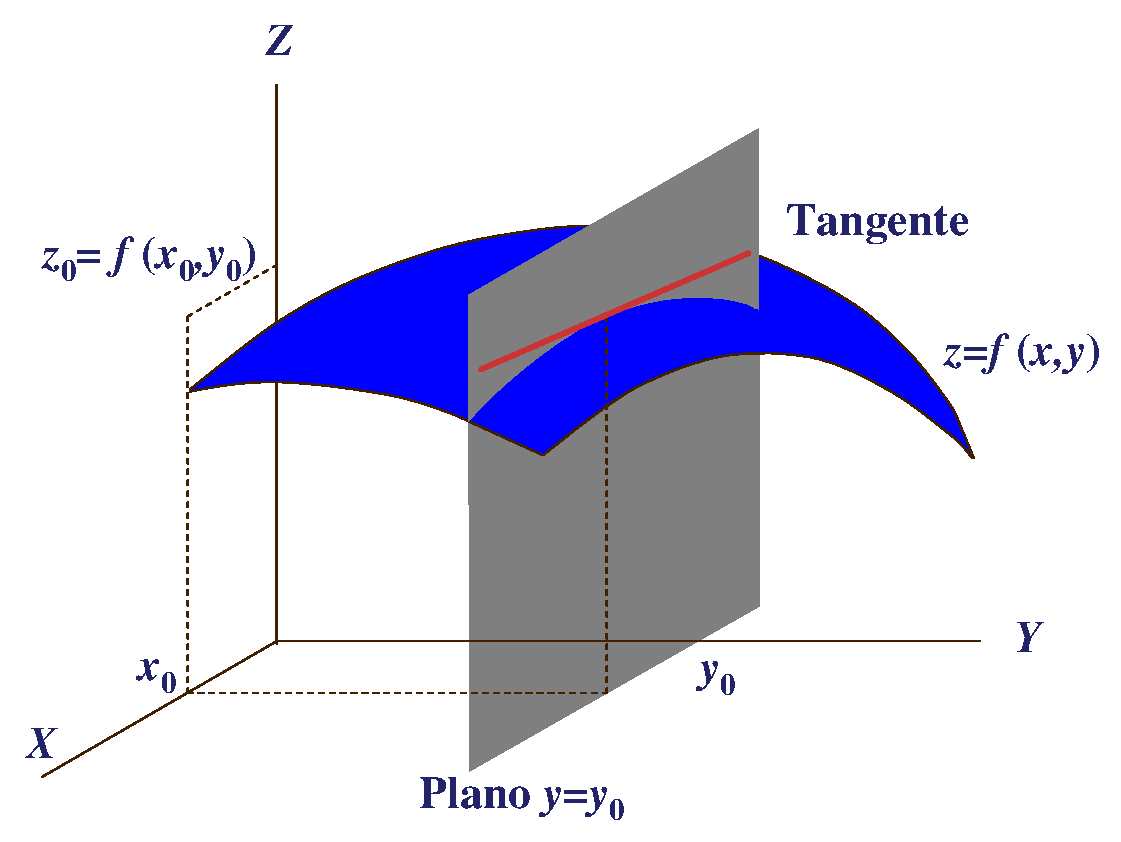
\includegraphics[scale=0.4]{img/derivadas_parciales/tangente_parcial.eps}
\caption{La derivada parcial de una función $f(x,y)$ con respecto a
$x$ en el punto $(x_0,y_0)$, como la pendiente de la recta tangente
a la curva descrita por la intersección de la superficie de $f$ y el
plano de ecuación $y=y_0$.}
\end{center}
\end{figure}


\subsection{Derivadas parciales sucesivas de una función de $n$
variables}

De la misma forma que en las funciones de una variable, mediante los
límites que las definen, siempre y cuando existan, obtenemos las
segundas, terceras y derivadas de cualquier orden. Es decir, si $f$
es una función real de $n$ variables, con sus correspondientes
derivadas parciales, a su vez también las mismas son funciones de
$n$ variables que, en determinadas condiciones, podrán derivarse de
nuevo con respecto a sus $n$ variables para obtener derivadas
parciales segundas, y así sucesivamente hasta órdenes superiores de
derivación.

Para la derivada parcial de segundo orden se utiliza la notación
$f_{x_ix_j}$ ó $\dfrac{{\partial ^2 f}} {{\partial x_j \partial x_i
}}$:


\[
f_{x_i x_j }  = \frac{{\partial ^2 f}} {{\partial x_j \partial x_i
}} = \frac{\partial } {{\partial x_j }}\left( {\frac{{\partial f}}
{{\partial x_i }}} \right)
\]

Por ejemplo, para una función de dos variables $f(x,y)$, tenemos dos
derivadas parciales de primer orden, que siguen siendo funciones de
las variables $x$ e $y$:

\[
\frac{{\partial f}} {{\partial x}}(x,y)\; ,\; \frac{{\partial f}}
{{\partial y}}(x,y)
\]
y cuatro diferentes de segundo orden, que también serán funciones de
$x$ e $y$, aunque ya no se refleje para aligerar la notación:


\[
\frac{\partial } {{\partial x}}\left( {\frac{{\partial f}}
{{\partial x}}} \right) = \frac{{\partial ^2 f}} {{\partial x^2 }}
\]

\[
\frac{\partial } {{\partial y}}\left( {\frac{{\partial f}}
{{\partial x}}} \right) = \frac{{\partial ^2 f}} {{\partial
y\partial x}}
\]


\[
\frac{\partial } {{\partial x}}\left( {\frac{{\partial f}}
{{\partial y}}} \right) = \frac{{\partial ^2 f}} {{\partial
x\partial y}}
\]

\[
\frac{\partial } {{\partial y}}\left( {\frac{{\partial f}}
{{\partial y}}} \right) = \frac{{\partial ^2 f}} {{\partial y^2 }}
\]

La primera y la última reciben el nombre de derivadas segundas,
mientras que la segunda y tercera se denominan derivadas cruzadas.

Si procedemos con las derivadas parciales de tercer orden tendríamos
ocho diferentes, y el número es más amplio con funciones de tres o
más variables. No obstante, el teorema conocido con \emph{Teorema de
Schwartz de las Derivadas Cruzadas} reduce el número de derivadas
parciales diferentes ya que afirma:

Si $f$ es una función de $n$ variables con derivadas parciales
segundas cruzadas continuas en un conjunto abierto que contiene al
punto $\vec{a}$, entonces en dicho punto se cumple

\[
\frac{{\partial ^2 f}} {{\partial x_i \partial x_j }} =
\frac{{\partial ^2 f}} {{\partial x_j \partial x_i }}
\]

e igual con las derivadas cruzadas de tercer y superior orden.

Es decir, si se cumplen las hipótesis del teorema de Schwartz
concluimos que, a efectos de cálculo, tan sólo importa el número de
veces que se deriva respecto a cada variable, pero no el orden de la
derivación.

\subsection{Vector gradiente y matriz hessiana}

Entre las múltiples aplicaciones de las derivadas parciales de
funciones de varias variables, destacan como herramientas
indispensables:

\begin{itemize}

\item El vector gradiente, muy utilizado, entre otras cosas, para determinar los puntos críticos de la
función, así como la dirección y sentido de máximo crecimiento de la
misma.

\item La matriz Hessiana, y su determinante, que se utilizan para
determinar el carácter de los puntos críticos de las funciones de
varias variables (máximos, mínimos y puntos silla).
\end{itemize}

\subsubsection*{Vector gradiente}
El conjunto de las $n$ derivadas parciales de una función de $n$
variables $f(x_1,x_2,\ldots,x_n)$, expresado en forma vectorial,
recibe el nombre de \emph{Vector Gradiente de $f$}. Es decir:

\[
\left(\frac{\partial f}{\partial x_1}(\vec a),\frac{\partial
f}{\partial x_2}(\vec a),\ldots,\frac{\partial f}{\partial x_n}(\vec
a)\right)
\]

El gradiente de $f$ también puede expresarse como la actuación de un
operador diferencial (entendemos como operador una expresión
matemática formal que tendrá sentido matemático una vez aplicado
sobre una función) llamado \emph{Operador Nabla}, que se nota como
$\vec\nabla$, sobre $f$. La expresión del operador nabla en
coordenadas cartesianas es:

\[
\vec {\nabla} =\left(\frac{\partial}{\partial x_1},\frac{\partial
}{\partial x_2},\ldots,\frac{\partial }{\partial x_n}\right)
\]

Con ello, el gradiente de $f$ toma la forma compacta:

\[
\left(\frac{\partial f}{\partial x_1},\frac{\partial f}{\partial
x_2},\ldots,\frac{\partial f}{\partial
x_n}\right)=\left(\frac{\partial}{\partial x_1},\frac{\partial
}{\partial x_2},\ldots,\frac{\partial }{\partial
x_n}\right)f=\vec{\nabla}f
\]


Y el gradiente de $f$ en el punto $\vec a$:

\[
\vec {\nabla} f(\vec a)
\]



\subsubsection*{Matriz hessiana}

Con el conjunto de todas las derivadas parciales segundas se define
la \emph{Matriz Hessiana} de una función $f(x_1,x_2,\ldots,x_n)$, y
se nota $H_f$, de tal manera que la fila $i$ es el vector gradiente
de la derivada parcial de $f$ con respecto a $x_i$, es decir:

\[
\renewcommand{\arraystretch}{2.2}
H_f=\left( {\vec \nabla \frac{{\partial f}} {{\partial x_1 }},\vec
\nabla \frac{{\partial f}} {{\partial x_2 }},...,\vec \nabla
\frac{{\partial f}} {{\partial x_n }}} \right)=\left(
\begin{array}{cccc}
 \dfrac{\partial^2 f}{\partial x_1^2}  & \dfrac{\partial^2 f}{\partial x_2\partial x_1}& \cdots & \dfrac{\partial^2 f}{\partial x_n\partial x_1}\\
 \dfrac{\partial^2 f}{\partial x_1\partial x_2} & \dfrac{\partial^2 f}{\partial x_2^2}  & \cdots & \dfrac{\partial^2 f}{\partial x_n\partial x_2} \\
                 \vdots                  &                 \vdots                  & \ddots &                 \vdots                  \\
 \dfrac{\partial^2 f}{\partial x_1\partial x_n} & \dfrac{\partial^2 f}{\partial x_2\partial x_n} & \cdots & \dfrac{\partial^2 f}{\partial x_n^2}  \\
\end{array}
\right)
\]

Con ello, la matriz Hessiana en $\vec a$:

\[
\renewcommand{\arraystretch}{2.2}
H_f(\vec a)=\left(
\begin{array}{cccc}
 \dfrac{\partial^2 f}{\partial x_1^2}( \vec a)  & \dfrac{\partial^2 f}{\partial x_2\partial x_1}(\vec a) & \cdots & \dfrac{\partial^2 f}{\partial x_n\partial x_1}(\vec a) \\
 \dfrac{\partial^2 f}{\partial x_1\partial x_2}(\vec a) & \dfrac{\partial^2 f}{\partial x_2^2}(\vec a)  & \cdots & \dfrac{\partial^2 f}{\partial x_n\partial x_2}(\vec a) \\
                 \vdots                  &                 \vdots                  & \ddots &                 \vdots                  \\
 \dfrac{\partial^2 f}{\partial x_1\partial x_n}(\vec a) & \dfrac{\partial^2 f}{\partial x_2\partial x_n}(\vec a) & \cdots & \dfrac{\partial^2 f}{\partial x_n^2}(\vec a)  \\
\end{array}
\right)
\]

Y al determinante de esta matriz, $\left| {H_f \left( {\vec a}
\right)} \right|$, se le llama \emph{Hessiano} de $f$ en $\vec a$.

\newpage

\section{Ejercicios resueltos}


\begin{enumerate}[leftmargin=*]
\item Dada la función $f(x)=\dfrac{x^3+x^2-2x-2}{x+3}$, se pide:
\begin{enumerate}

\item Calcular la tasa de variación media de $f$ en los intervalos
$[-1,3]$, $[-1,0]$ y $[-1,-0.5]$, y calcular las correspondientes
rectas secantes.

\begin{indicacion}
{
\begin{enumerate}
\item Para calcular la tasa de variación media, definir
previamente la función, y luego, por ejemplo para el intervalo
$[-1,3]$, aplicamos la fórmula vista en la teoría:

\[
\textrm{TVM} f[-1,3]=\frac{\Delta y}{\Delta
x}=\frac{f(3)-f(-1)}{3-(-1)}.
\]

\item Para calcular la ecuación de la recta secante, podemos
utilizar, por ejemplo, la ecuación de la recta de la que conocemos
un punto por el que pasa, $(x_0,y_0)$ y su pendiente, $m$:


\[
y - y_0  = m\left( {x - x_0 } \right)
\]

En nuestro caso, para el primero de los intervalos considerados, el
punto puede ser, por ejemplo el $(-1,f(-1))$; y la pendiente viene
dada por la tasa de variación media de la función en dicho
intervalo. Es decir, la recta que buscamos tendrá como ecuación:


\[
y - f( - 1) = \textrm {TVM} f[ - 1,3]\left( {x - ( - 1)} \right)
\]

\item Después de calcular la ecuación de la recta secante, podemos
comprobar que la misma corta a la función en los puntos adecuados
sin más que representar en la misma gráfica tanto $f$ como la recta
calculada.

\end{enumerate}
}
\end{indicacion}


\item Calcular la tasa de variación instantánea de $f$ en el punto
$-1$ haciendo uso de límites, y calcular la correspondiente recta
tangente.

\begin{indicacion}
{
\begin{enumerate}
\item Como ya sabemos por la teoría, las tasa de variación
instantánea de la función en un punto dado si existe, recibe el
nombre de derivada de la función en el punto, y se calcula mediante
el límite:


\[
f'(a) = \mathop {\lim }\limits_{h \to 0} \frac{{f(a + h) - f(a)}}
{h}
\]
en donde, por aligerar la notación, hemos llamado $h$ a lo que en la
teoría denominábamos $\Delta x$.

Por lo tanto, para calcular la derivada de la función $f$ en $a=-1$
mediante la definición, procedemos con:

\[
f'(-1) = \mathop {\lim }\limits_{h \to 0} \frac{{f(-1 + h) - f(-1)}}
{h}
\]

Para calcular el límite, podemos utilizar el botón \boton{Calcular
un límite} de la barra de botones.

\item Para el cálculo de la recta tangente, de nuevo sabemos que
la misma pasa por el punto $(-1, f(-1))$, y que su pendiente vale
$f'(-1)$. Por lo tanto su ecuación es:

\[
y - f( - 1) = f'(-1)\left( {x - ( - 1)} \right)
\]

\item De nuevo, conviene representar en la misma gráfica tanto la
función como la recta tangente en el punto considerado, para
comprobar que los cálculos han sido los correctos.

\end{enumerate}
}
\end{indicacion}


\end{enumerate}




\item Estudiar mediante la definición de derivada la derivabilidad
de las funciones siguientes:


\[
f(x)=|x-1| \quad \textrm{en $x=1$,}
\]
\[
g(x)=\left\{%
\begin{array}{ll}
   x \sen\dfrac{1}{x}, & \hbox{si $x\neq 0$;} \\
   0, & \hbox{si $x=0$.} \\
\end{array}%
\right. \quad \textrm{en $x=0$.}
\]

\begin{indicacion}
{
\begin{enumerate}
\item Para la función $f(x)$, podemos inicialmente definirla,
teniendo en cuenta que la sintaxis de la función valor absoluto es
$\comando{Abs}$, y después utilizar la definición de derivada en un
punto dada en el problema anterior, y calcular el límite mediante el
botón \boton{Calcular un límite}. Por lo tanto, si existe la
derivada en $x=1$ su valor es:


\[
f'(1) = \mathop {\lim }\limits_{h \to 0} \frac{{f(1 + h) - f(1)}}
{h}
\]

\item Para la función $g(x)$, podemos, para su definición,
utilizar la función condicional de Derive
\comando{If(condición,opción 1,opción 2)}, de tal forma que si se
cumple la \comando{condición} el programa realizará la
\comando{opción 1}, y si no se cumple realizará la \comando{opción
2}. La función condicional de Derive, \comando{If}, entre otras
muchas posibilidades, sirve para introducir funciones definidas a
trozos. En nuestro caso la \comando{condición} es $x\neq y$, la
\comando{opción 1} es $x\sin(1/x)$, y la \comando{opción 2} es $0$.

Así, la función $g(x)$ puede definirse mediante:

\[
g(x):=\comando{IF}(x\neq0,x\sin(1/x),0)
\]


Y con ello, para calcular la derivada en $x=0$, procedemos mediante
la definición de derivada en un punto:


\[
g'(0) = \mathop {\lim }\limits_{h \to 0} \frac{{g(0 + h) - g(0)}}
{h}
\]



\end{enumerate}
}
\end{indicacion}


\item  Calcular las derivadas de las siguientes funciones hasta el
orden 4:

\begin{enumerate}
\item  $a^x\log a$.

\item  $\dfrac{\sen x +\cos x}{2}$.

\item  $\dfrac{1}{\sqrt{1+x}}$.
\end{enumerate}

A la vista de los resultados, ¿cual sería la expresión de la
derivada $n$-ésima de cada una de estas funciones?

\begin{indicacion}
{
\begin{enumerate}
\item Para cada una de las funciones, introducir la expresión de
la misma, y proceder al cálculo de la sucesivas derivadas, desde
orden 1 hasta orden 4, utilizando, por ejemplo, el botón
\boton{Hallar una derivada} de la barra de botones, escogiendo el
orden adecuado.

\item Para el cálculo de la derivada $n$-ésima, teniendo en cuenta
que en el cuadro de diálogo que aparece al pinchar en el botón
\boton{Hallar una derivada} tan sólo podemos introducir como orden
de la misma un número entero, pero nunca un parámetro como $n$, no
queda otra posibilidad que proceder por inducción, y a la vista de
las primeras derivadas suponer cuál sería el valor de la derivada de
orden $n$. Posteriormente, podemos comprobar que nuestra suposición
es correcta utilizando la fórmula que hemos encontrado para calcular
una derivada de orden bastante alto y comparando con el valor que da
Derive para esa misma derivada.

\end{enumerate}
}
\end{indicacion}
\item  Dada la función:
\[
g(x)=\dfrac{2x^{3}-3x}{x^{2}+1}
\]

\begin{enumerate}
\item  Representar la gráfica de $g$.

\begin{indicacion}
{Una vez introducida la función en Derive, utilizar el botón
\boton{Ventana 2D} para pasar al entorno de dibujo de funciones de
una única variable, y allí utilizar el botón \boton{Representar
Expresión} para representar la gráfica. }
\end{indicacion}

\item  Calcular la función derivada $g^{\prime }(x),$ y representar su
gráfica.

\begin{indicacion}
{Marcar la expresión de la función y utilizar el botón \boton{Hallar
una derivada} y escoger la variable $x$ y el orden 1. Para
representar la gráfica de la función derivada, seguir el proceso del
punto anterior. }
\end{indicacion}

\item  Calcular las raíces de $g^{\prime }(x).$

\begin{indicacion}
{Para calcular las raíces, marcar la expresión de la función
derivada y utilizar el botón \boton{Resolver o despejar}, escogiendo
la variable $x$, y conviene utilizar el dominio Real para obtener
únicamente la raíces reales, que son las que nos interesan.

}
\end{indicacion}

\item  A la vista de las raíces y de la gráfica de la función
derivada, determinar los extremos relativos de la función y los
intervalos de crecimiento.

\begin{indicacion}
{Tener en cuenta que la función es creciente en los puntos en los
que la derivada es positiva, decreciente si la derivada es negativa,
y aquellos puntos en los que la derivada vale cero (puntos críticos)
serán extremos relativos si en ellos cambia el crecimiento de la
función. }
\end{indicacion}

\item Calcular la segunda derivada $g''(x),$ y representar su
gráfica.

\begin{indicacion}
{La podemos obtener derivando, mediante el botón \boton{Hallar una
derivada}, la función de partida, y escogiendo como orden de
derivación 2; o también podemos directamente derivar la función
derivada escogiendo como orden de derivación 1. Para representar la
gráfica seguimos los pasos de cualquier otra representación.

}
\end{indicacion}

\item  Calcular las raíces de $g''(x).$

\begin{indicacion}
{Igual que en apartados anteriores, marcamos la expresión de la
segunda derivada y utilizamos el botón \boton{Resolver o despejar}.

}
\end{indicacion}

\item  A la vista de las raíces y de la gráfica de la segunda
derivada, determinar los intervalos de concavidad de la función y
los puntos de inflexión.

\begin{indicacion}
{Recordar que la función de partida es cóncava si la derivada
segunda es mayor que 0, convexa si la derivada segunda es menor que
0, y en los puntos en los que valga cero hay un candidato a punto de
inflexión, que confirmaremos si lo es viendo si la función cambia de
concavidad en dicho punto.

}
\end{indicacion}

\end{enumerate}

\item Estudiar el crecimiento, la concavidad, los extremos
relativos y los puntos de inflexión de la función:

\[
f(x)=\dfrac{x}{x^2-2}
\]


\begin{indicacion}
{
\begin{enumerate}
\item Calcular la primera derivada (botón \boton{Hallar una
derivada}) y encontrar sus raíces (botón \boton{Resolver o
despejar}). Con ello podemos determinar los intervalos de
crecimiento y decrecimiento y los extremos relativos, si los hay
(puede suceder que no encontremos raíces de la función derivada).

\item De igual forma, proceder al cálculo de la segunda derivada y
de sus raíces para determinar concavidad, convexidad y puntos de
inflexión.

\item Puede resultar muy ilustrativo representar tanto la gráfica
de la función de partida como las de su primera y segunda derivada
para corroborar las conclusiones de los apartados anteriores.

\end{enumerate}
}
\end{indicacion}

\item  Calcular las siguientes derivadas parciales:

\begin{enumerate}

\item  $\dfrac{\partial }{\partial V}\dfrac{nRT}{V}.$

\begin{indicacion}
{
\begin{enumerate}

\item Introducir la expresión en Derive.

\item Utilizar el botón \boton{Hallar una derivada}, desplegando
la lista de hipotéticas variables en las que podemos derivar
(evidentemente, para Derive tanto $n$ como $R$ también son
variables), y escoger la variable $V$ y el orden $1$.

\end{enumerate}
}
\end{indicacion}

\item  $\dfrac{\partial ^{2}}{\partial x\partial y}e^{x+y}\ $sen$\ \dfrac{x}{%
y}.$


\begin{indicacion}
{
\begin{enumerate}

\item Introducir la expresión en Derive. Tener en cuenta la
sintaxis adecuada de la función seno: \comando{sin}.

\item Utilizar el botón \boton{Hallar una derivada}, desplegando
la lista de hipotéticas variables en las que podemos derivar y
escoger la variable $y$ y el orden $1$. Con ello, obtenemos la
primera derivada con respecto a $y$.

\item Una vez obtenida primera derivada con respecto a $y$, para
obtener la segunda con respecto a $x$, marcamos la expresión
obtenida en el apartado anterior y volvemos a derivarla (botón
\boton{Hallar una derivada}) pero con respecto a $x$, escogiendo
como orden de derivación el $1$.


\end{enumerate}
}
\end{indicacion}

\item  $\dfrac{\partial ^{3}}{\partial y\partial x^2}e^{x+y}\ $sen$\ \dfrac{x}{%
y}.$

\begin{indicacion}
{
\begin{enumerate}

\item Como ya tenemos la expresión de la función introducida para
el apartado anterior, la marcamos y pasamos directamente a la
derivación.

\item En primer lugar realizamos la derivada de segundo orden con
respecto a $x$. Para ello, botón \boton{Hallar una derivada},
escoger como variable de derivación $x$ y como orden $2$.

\item Para la derivada de orden 3, partiendo de la expresión
generada en el apartado anterior, volvemos a derivar pero ahora con
respecto a $y$ y de orden 1.

\end{enumerate}
}
\end{indicacion}

\end{enumerate}

\item  Dada la función
\[
f(x,y,z)=\ \sen \left( \left( x^{2}-y^{2}\right) z\right)
\]
\begin{enumerate}

\item Definir la función en Derive y calcular $f(0,-1,\pi/2)$.


\begin{indicacion}
{
\begin{enumerate}

\item Para definirla, tan sólo introducir la expresión con su
correspondiente operador de definición y la sintaxis adecuada de la
función seno:

\[
f(x,y,z):=\sin((x^2-y^2)z)
\]

\item Una vez definida, para calcular $f(0,-1,\pi/2)$, introducir
directamente la expresión en la línea de edición y simplificar.

\end{enumerate}
}
\end{indicacion}

\item Calcular su vector gradiente.

\begin{indicacion}
{Para calcular su vector gradiente, utilizar la función
$\comando{GRAD}$, indicando también las variables en las que se
realizarán las derivadas parciales:

\[
\comando{GRAD}(F(x,y,z), [x,y,z])
\]

}
\end{indicacion}

\item Calcular su matriz Hessiana.

\begin{indicacion}
{Para calcular la matriz Hessiana, aplicar de nuevo el gradiente
sobre la expresión del gradiente calculado en el apartado anterior.
Para ello, simplemente marcar la expresión anterior y volver a
aplicar el gradiente, o directamente:
$\comando{GRAD}(\comando{GRAD}(F(x,y,z),[x,y,z]),[x,y,z])$

}
\end{indicacion}

\item Comprobar que se cumple el teorema Schwartz de las derivadas
para las derivas cruzadas, calculando:

\begin{enumerate}

\item $\dfrac{{\partial ^3 f}} {{\partial x\partial z\partial y}}$

\item $\dfrac{{\partial ^3 f}} {{\partial z\partial x\partial y}}$

\item ¿Puedes predecir el valor de: $\dfrac{{\partial ^3 f}}
{{\partial y\partial x\partial z}}$?

\end{enumerate}

\begin{indicacion}
{
\begin{enumerate}

\item Para el primero de los apartados, calcular, mediante el
botón \boton{Hallar una derivada}, en primer lugar la derivada de
orden 1 con respecto a $y$. A continuación derivar, con orden de
derivación 1, la expresión resultante con respecto a $z$. Y
posteriormente derivar, de nuevo con orden 1, con respecto a $x$.

\item Para el segundo de los apartados, proceder como en el
primero pero cambiando el orden de derivación: en primer lugar con
respecto a $y$, luego con respecto a $x$, y por último con respecto
a $z$. Observar cómo, a pesar de haber cambiado el orden de
derivación, el resultado final no ha variado.

\item En el último de los apartados, se puede predecir fácilmente
que el resultado será el mismo, ya que únicamente hemos cambiado el
orden de derivación. No obstante, puede comprobarse fácilmente.

\end{enumerate}

}
\end{indicacion}


\end{enumerate}
\end{enumerate}


\section{Ejercicios propuestos}

\begin{enumerate}[leftmargin=*]

\item  Probar que no es derivable en $x=0$ la siguiente función:
\[ f(x)=\left\{
\begin{array}{ccl}
    e^x-1 &  & \mbox{si } x\geq 0,  \\
    x^3 &  & \mbox{si } x<0.
\end{array}\right.
\]

\item  Para cada una de las siguientes curvas, hallar las ecuaciones
de las rectas tangente y normal en el punto $x_{0}$ indicado.
\begin{enumerate}
    \item  $y=x^{\sen x},\quad x_{0}=\pi/2$.

    \item  $y=(3-x^2)^4\sqrt[3]{5x-4},\quad x_{0}=1$.

    \item  $y=\log \sqrt{\dfrac{1+x}{1-x}}+\arctg x, \quad x_{0}=0$.
\end{enumerate}

\item Una nave espacial está en problemas cerca del sol. Se
encuentra en la posición $(1,1,1)$ y la temperatura de la nave cuando
está en la posición $(x,y,z)$ viene dada por
$T(x,y,z)=\mbox{e}^{-x^2-2y^2-3z^2}$ donde $x,y,z$ se miden en metros.
¿En qué dirección debe moverse la nave para que la temperatura decrezca
lo más rápidamente posible?
\end{enumerate}